\documentclass{article}

% if you need to pass options to natbib, use, e.g.:
%     \PassOptionsToPackage{numbers, compress}{natbib}
% before loading neurips_2024


% ready for submission
\usepackage[final]{neurips_2024}


% to compile a preprint version, e.g., for submission to arXiv, add add the
% [preprint] option:
%     \usepackage[preprint]{neurips_2024}


% to compile a camera-ready version, add the [final] option, e.g.:
%     \usepackage[final]{neurips_2024}


% to avoid loading the natbib package, add option nonatbib:
%    \usepackage[nonatbib]{neurips_2024}


\usepackage[utf8]{inputenc} % allow utf-8 input
\usepackage[T1]{fontenc}    % use 8-bit T1 fonts
\usepackage{hyperref}       % hyperlinks
\usepackage{url}            % simple URL typesetting
\usepackage{booktabs}       % professional-quality tables
\usepackage{amsfonts}       % blackboard math symbols
\usepackage{nicefrac}       % compact symbols for 1/2, etc.
\usepackage{microtype}      % microtypography
\usepackage{xcolor}         % colors

\usepackage{amsmath}
\usepackage{amsfonts}
\usepackage{amssymb}
\usepackage{mathtools}

\usepackage{titlesec}

\setcounter{secnumdepth}{4}

\titleformat{\paragraph}
{\normalfont\normalsize\bfseries}{\theparagraph}{1em}{}
\titlespacing*{\paragraph}
{0pt}{3.25ex plus 1ex minus .2ex}{1.5ex plus .2ex}



\title{2024/25 PHYS4036 MLiS2 Project Report}

\author{%
  Sam Tam \\
  School of Physics and Astronomy\\
  University of Nottingham\\
  Nottingham, NG7 2RD \\
  \texttt{ppxst5@nottingham.ac.uk}
}


\begin{document}


\maketitle


\begin{abstract}
  This project aims to develop machine learning models to predict the speed and steering angle of images captured by Raspberry Pi cars. The project is divided into two parts: an online challenge and a live test. Multiple models with convolutional neural networks followed by fully connected layers were developed using transfer learning from pre-trained models. The models achieved a mean-squared-error of 0.009 in the public leaderboard and a mean-squared-error of 0.011 in the private leaderboard, and secured first place in the online challenge, demonstrating excellent predictive accuracy and generalisability. In the live test, the model successfully completed 90\% of the tasks, including lane following and stop-on-object, though some challenges remain. Future studies could focus on enhancing data collection for better generalisability and upgrading Raspberry Pi cars' hardware for higher image resolution and greater model complexity.
\end{abstract}

\section{Introduction}
In the recent decade, autonomous driving has become one of the most rapidly advancing areas in the field of artificial intelligence (AI). Numerous companies have been founded with the goal of developing reliable self-driving systems \citep{Law_2023}. As the technology matures, hands-on experience has become more valuable for students and researchers to deepen their understanding of how real-world AI applications work.

One accessible platform for gaining such experience is PiCar \citep{SunFounder}. PiCar is a small robot car that equipped with an onboard camera to capture forward-facing perspective of the car's environment, and a Raspberry Pi (RPi) single-board computer \citep{RaspberryPi} for real-time computation. The captured image frames can be used as input to machine learning models running on the RPi that predict control signals, including steering angle and speed, of the car.

This project is divided into two phrases: an online challenge and a live test. In the online challenge, provided data were used to train the models for predicting the car's steering angle and speed of a given image. In the live test, models were trained on data collected by me, and the models were deployed to the PiCar to complete a variety of tasks to assess the model's performance.

The report is divided into five sections: introduction, methods, results, discussion, and conclusion. Section 2 (Methods), 3 (Results), and 4 (Discussion) are further divided into two subsections, corresponding to the online challenge and the live test phrase of the project.


\section{Methods}
In both phases of the project — the online challenge and the live test — the objective was to predict the PiCar's steering angle and speed from images captured by its onboard camera. Both control signals were normalised to the range \([0, 1]\) using the following formulas \citep{Kaggle}:

\[
  \text{angle}_{\text{norm}} = \frac{\text{angle} - 50}{80}
  \quad \text{where } \text{angle} \in [90 - 40, 90 + 40] = [50, 130]
\]

\[
  \text{speed}_{\text{norm}} = \frac{\text{speed} - 0}{35}
  \quad \text{where } \text{speed} \in [0, 100]
\]

Here, the steering angle is centred at 90 (with a range of ±40), and the recorded speed in the dataset is either \(0 \text{ or } 35\). \(\text{angle}_{\text{norm}} = 0\) corresponds to a fully left turn, and \(\text{angle}_{\text{norm}} = 1\) corresponds to a fully right turn. The normalised angles were restricted to steps of \(1/16 = 0.0625\), resulting in 17 possible angle values. Similarly, \(\text{speed}_{\text{norm}} = 0\) indicates the car stopped, and \(\text{speed}_{\text{norm}} > 0\) represents the car moved. Note that the PiCar is capable of running at any integer speed in range [0, 100], but only two speed values, 0 and 35, were used during the data collection period to restrict the normalised speed to either 0 (stop) or 1 (move).



\subsection{Online challenge}

The online challenge was assessed by the mean squared error (MSE) of a test dataset's private leaderboard, where a lower value indicated better model performance.

The steering angle model and the speed model were trained separately, to reduce the complexity of data preprocessing and modelling.

\subsubsection{Training data}

There were 13.8k RGB images of resolution 240 x 320 provided with the corresponding normalised labels \citep{Kaggle}. The dataset was noisy and included inaccurate labels, missing labels, and invalid image files. Figure \ref{fig:inaccurate_label} shows some examples of inaccurate labelling.

\begin{figure}[h]
  \centering
  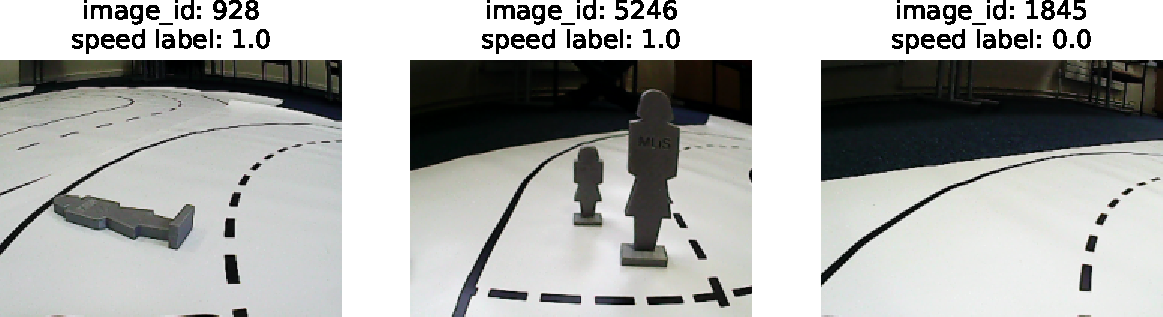
\includegraphics[width=0.8\textwidth]{figures/inaccurate_label.pdf}
  \caption{Examples of inaccurate labels in the dataset.}
  \label{fig:inaccurate_label}
\end{figure}

\paragraph{Data cleaning}
In order to clean the dataset, first I wrote a Python script to read all the images, to handle errors, and to remove image files that caused errors. After that I ensured all the labels were within the range of [0, 1], and each record contained complete labels for both steering angle and speed.

\paragraph{Training set and test set}
\label{sec:train_test_split}
The data were split into training set and test set, with a ratio of 0.85 : 0.15, using explicitly defined random seeds to assure the reproducibility of the results, and the ratio between classes in both sets was approximately the same.

\paragraph{Data distribution}
I visualised the data distribution in Figure \ref{fig:angle_speed_distribution}. It shows that the distribution of steering angles is left-skewed and non-uniform, and the distribution of speeds is imbalanced, roughly 25:75.

\begin{figure}[h]
  \centering
  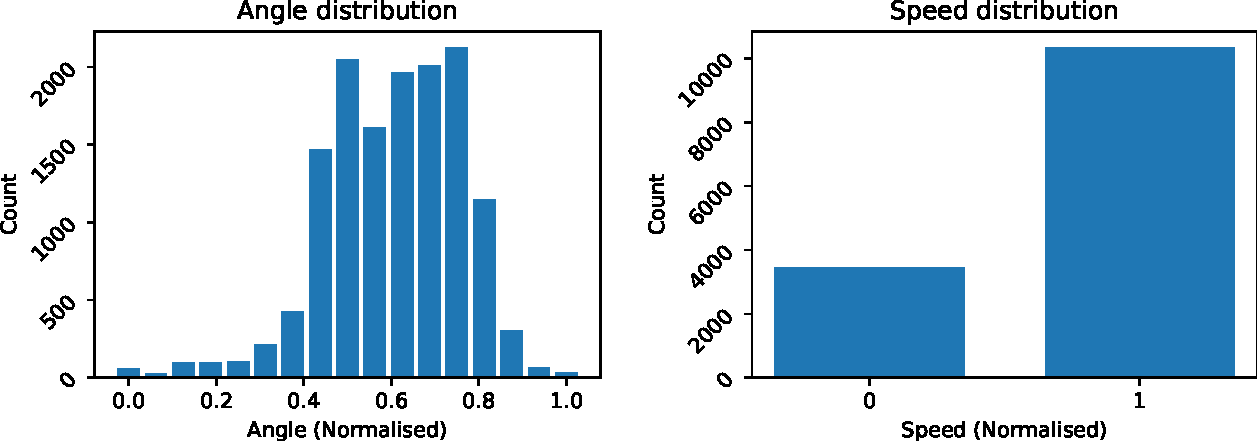
\includegraphics[width=0.9\textwidth]{figures/angle_speed_distribution.pdf}
  \caption{Distribution of steering angles and speeds in the dataset.}
  \label{fig:angle_speed_distribution}
\end{figure}

\paragraph{Data balancing}
Given the severe class imbalance in steering angle, I applied a combination of oversampling and undersampling to the dataset, leading to a ratio between a minority and a majority class of approximately 0.22 : 0.78. The above ratio was chosen carefully for several reasons:
\begin{itemize}
  \item Oversampling too aggressively duplicated the minority classes too much, which led to overfitting.
  \item Undersampling too aggressively reduced the majority classes too much, which led to missing information of the majority class and underfitting.
\end{itemize}
After some experimenting, the above ratio turned out to be the best choice.

I left the speed dataset unchanged and used weighted loss to address the class imbalance instead, as it was not highly imbalanced.

Figure \ref{fig:angle_speed_distribution_balanced} shows the distribution of steering angles and speeds after balancing.

\begin{figure}[h]
  \centering
  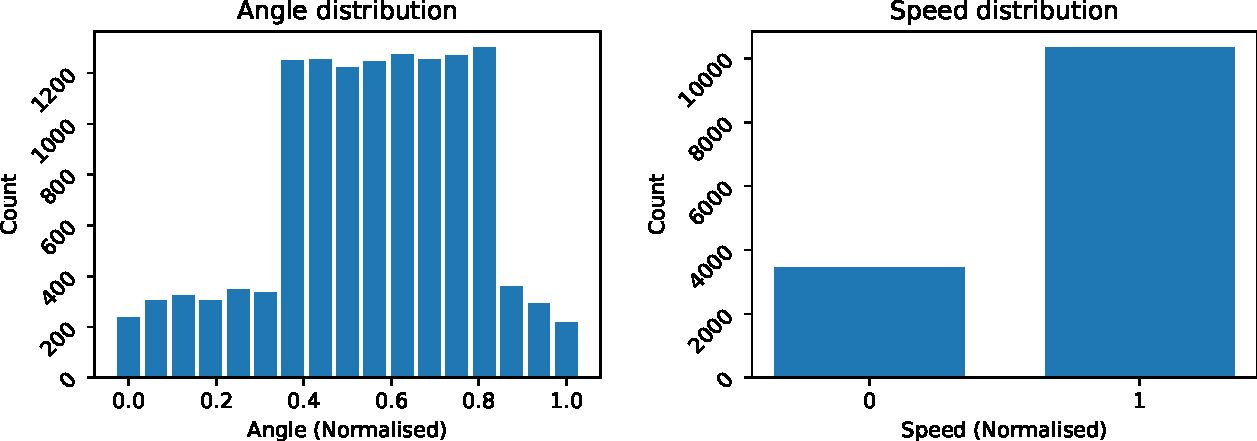
\includegraphics[width=0.9\textwidth]{figures/angle_speed_distribution_balanced.pdf}
  \caption{Distribution of steering angles and speeds after balancing.}
  \label{fig:angle_speed_distribution_balanced}
\end{figure}

\paragraph{Data augmentation}
To increase the data variety and improve the generalisability of the model, I applied data augmentation to the training set to mimic real-world conditions, such as changes in lighting, movements of camera, and positioning of the PiCar. I augmented the images by applying the following settings randomly:
\begin{itemize}
  \item Brightness scaled by factor in range [0.7, 1.3]
  \item Contrast scaled by factor in range [0.75, 1.25]
  \item Hue scaled by factor in range [0.95, 1.05]
  \item Saturation scaled by factor in range [0.7, 1.2]
  \item JPEG compression quality scaled by factor in range [0.8, 1.0]
  \item Rotation: [-5\textdegree, 5\textdegree]
  \item Crop to size of 210 x 280 randomly
\end{itemize}
, and resized the images back to the original size. Figure \ref{fig:augmentation} shows some samples of the augmentation.

\begin{figure}[h]
  \centering
  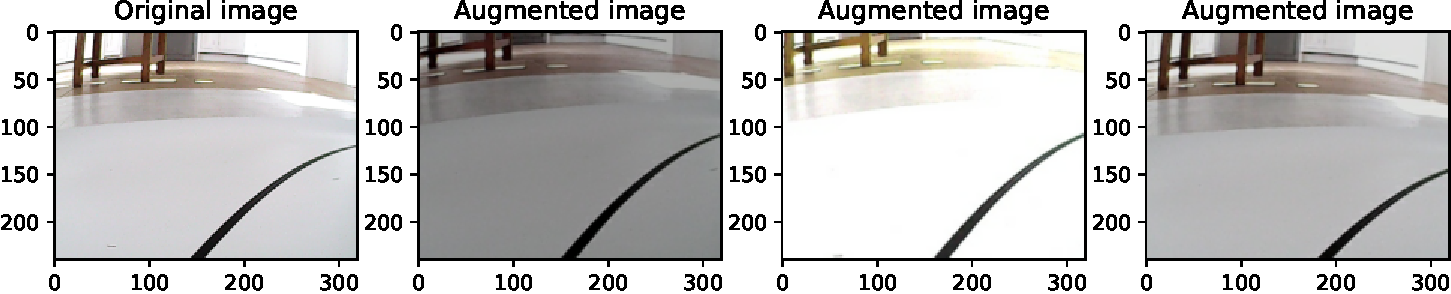
\includegraphics[width=0.9\textwidth]{figures/augmentation.pdf}
  \caption{Samples of augmented images.}
  \label{fig:augmentation}
\end{figure}

\subsubsection{Modelling}
The steering angle model and the speed model were trained separately.

Transfer learning was used to train the models. The base model for both the steering angle and speed models was pre-trained on MobileNetV3Large, which provided a good balance between feature extracting complexity and efficiency. The base model was frozen to prevent overfitting. Each model was followed by 10 heads - sub-models that took the features extracted from the base model as the input and outputted the steering angle or speed. These heads had different structures, which could include convolutional layers, global average pooling layer, flatten layer, fully connected layers, and dropout layers. The use of varied head architectures aimed to capture diverse features from the images, thereby increasing model generalisability and improving prediction accuracy.

Figure \ref{fig:angle_heads} and Figure \ref{fig:speed_heads} show the structure of the heads.

\paragraph{Structures and hyperparameters}
The structures of the heads were randomly created using the following rules:
\begin{itemize}
  \item Number of convolutional layers: \{0, 1, 2\}
  \item Number of global average pooling layers: \{0, 1\}
  \item Number of flatten layers: 1 - number of global average pooling layers
  \item Number of fully connected layers: \{0, 1, 2, 3, 4\}
\end{itemize}
Dropout layers were added based on observed overfitting during training.

The hyperparameters of the layers in the models were chosen and tuned manually based on observed training and test loss.

\paragraph{Training}

The models were trained for 50 epochs with batch size of 64 and Adam optimiser with decaying learning rate:
\[
  \begin{aligned}
    \text{learning\_rate} =
    \begin{cases}
      0.02,                                                                                                         & \text{if epoch = 0}
      \\
      \max\left(\frac{\text{initial\_learning\_rate}}{1 + \left(\frac{\text{epoch} - 1}{3}\right) \times \text{decay\_rate}}, 0.00015\right), & \text{otherwise}
    \end{cases}
    \\
    \text{where } \text{initial\_learning\_rate} = 0.01 \text{ and } \text{decay\_rate} = 0.4
  \end{aligned}
\]
The above decaying learning rate strategy aimed to keep the first epochs' learning rate high to improve convergence rate, while gradually decreased the learning rate to prevent overshooting.

The models were trained using the following loss functions:
\begin{itemize}
  \item Steering angle model: Mean squared error
  \item Speed model: Weighted mean squared error
\end{itemize}

During the training of the steering angle models, the training data was randomly selected and augmented from the training set every epoch to reduce the risk of overfitting and introduce diversity of augmented images and undersampled classes.


\subsubsection{Prediction}
To further increase the generalisability of the predictions, 4 models were trained with different random seeds for the train/test split. As a result, each image had \( 4 \times 10 = 40 \) predicted values for the steering angle and the speed. The predicted values were then averaged to obtain the prediction.

A threshold \(\text{speed}_\text{threshold}\) was introduced to the speed prediction to reduce the mean squared error (MSE) and was tuned using the test set. The speed prediction was adjusted as follows:

\[
  \begin{aligned}
    \text{adjusted speed prediction} =
    \begin{cases}
      0.5 \times \operatorname{sign}(\tilde{y}) + 0.5, & \text{if } |\tilde{y}| > \text{speed}_\text{threshold} \\
      \tilde{y} + 0.5,                                 & \text{otherwise}
    \end{cases}
    \\
    \text{where } \tilde{y} = \text{original speed prediction} - 0.5
  \end{aligned}
\]

A manual inspection was carried out on the predictions with high variance between the 40 predicted values to remove clearly incorrect predictions.



\begin{figure}[h]
  \centering
  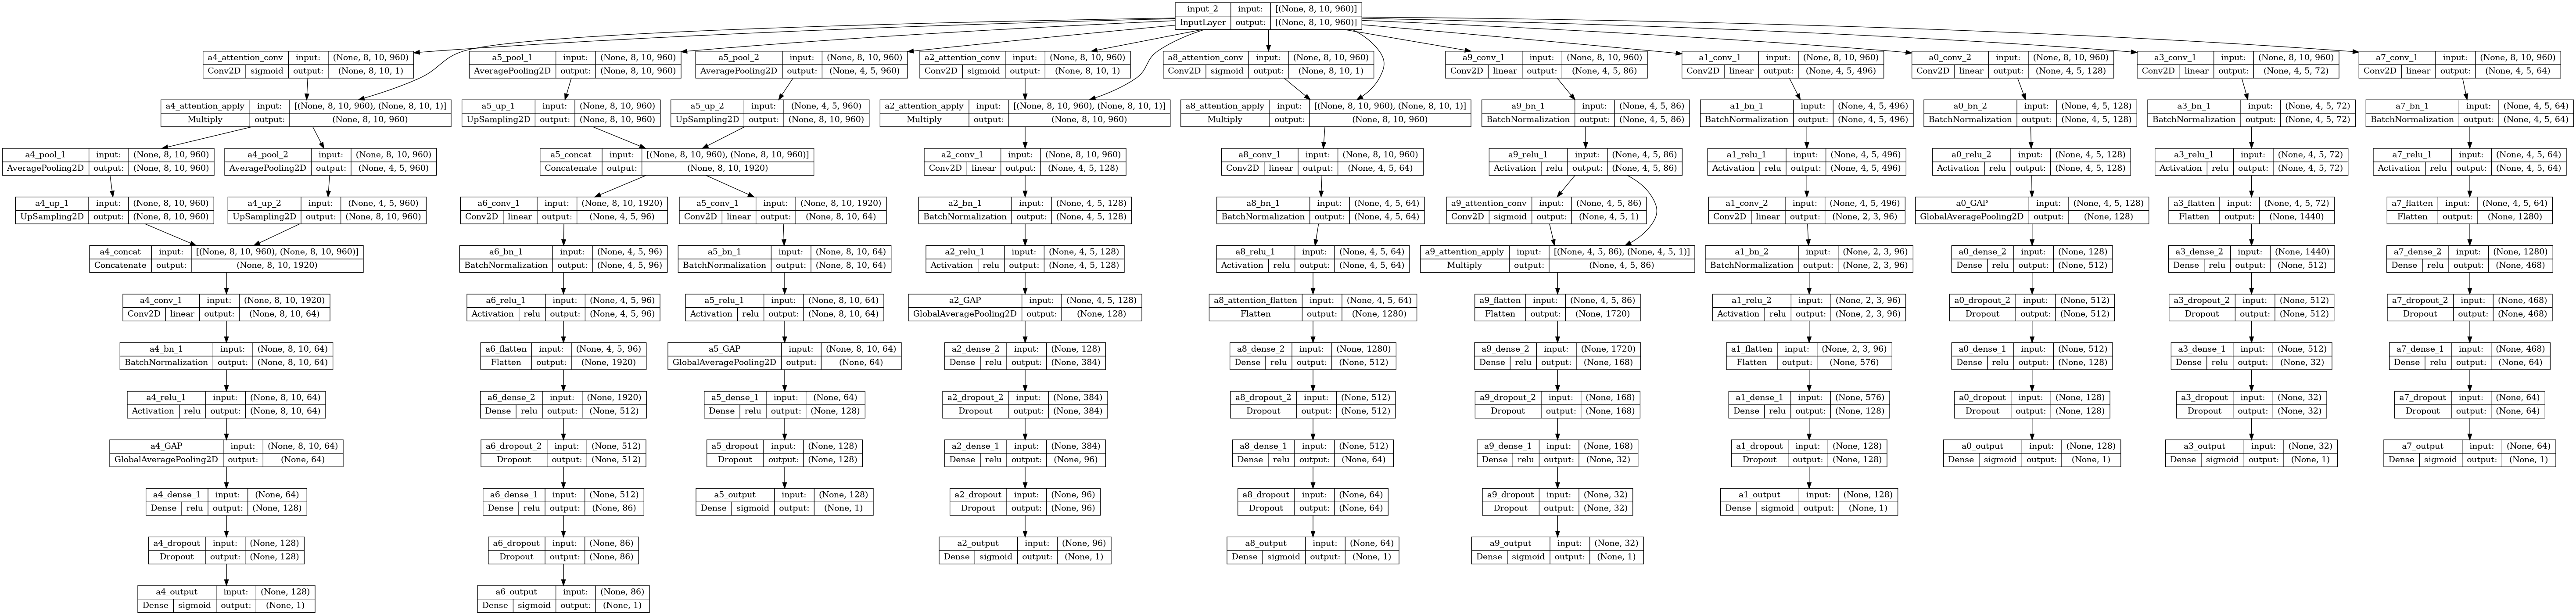
\includegraphics[width=0.9\textwidth]{figures/angle_heads.png}
  \caption{Structure of the steering angle model's heads.}
  \label{fig:angle_heads}
\end{figure}

\begin{figure}[h]
  \centering
  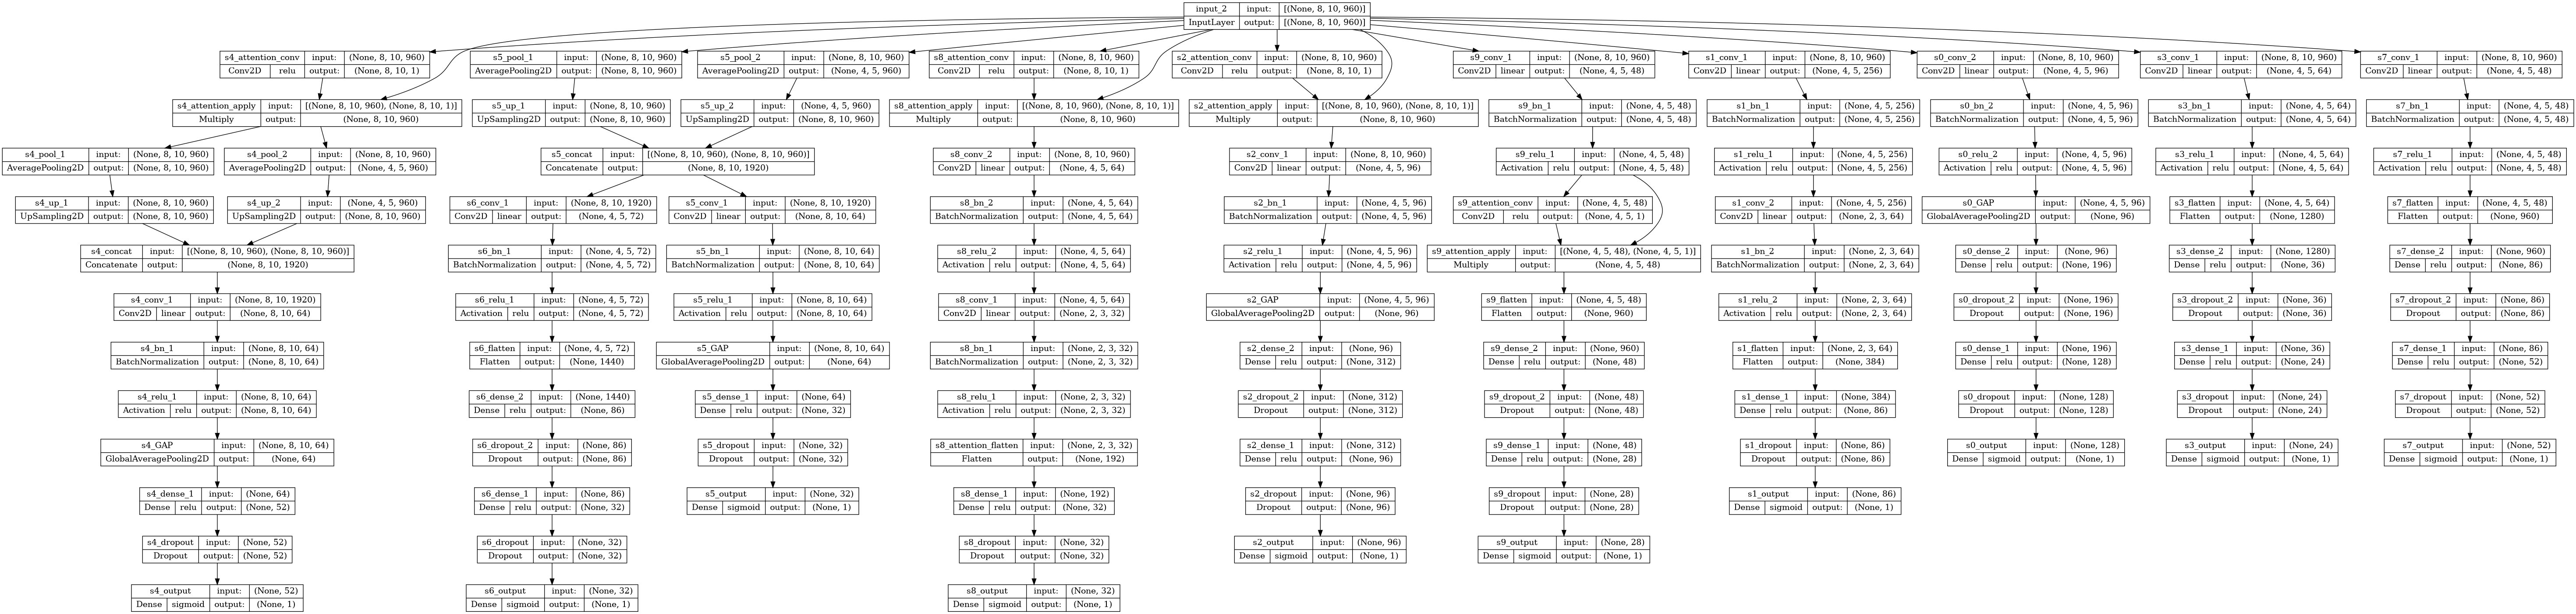
\includegraphics[width=0.9\textwidth]{figures/speed_heads.png}
  \caption{Structure of the speed model's heads.}
  \label{fig:speed_heads}
\end{figure}


\subsection{Live test}
The live test performance was assessed by the PiCar's ability to complete a variety of tasks, such as driving along the road and stopping on pedestrians or obstacles ahead. The trained model was loaded onto a pre-build PiCar. 

\subsubsection{Training data}

\paragraph{Data collection and data cleaning}
To maintain the consistency of the training data's driving logic, 16.8k driving data was collected from scratch. The data was collected in the following ways:
\begin{itemize}
  \item Capture the PiCar's video feed and control signals while driving along all three maps according to the rules \citep{Kaggle}.
  \item Train the model on the collected data and deploy the model to the PiCar.
  \item Collect more data to reinforce the weak points. E.g.: 
  \begin{itemize}
    \item Collect more data of turning left in the oval track if the PiCar turned left poorly.
    \item Collect more data of stopping on pedestrians when turning if the PiCar did not stop on pedestrians in a turn.
    \item Collect more data of stopping at a red light if the PiCar did not stop at a red light.
  \end{itemize} 
  \item Retrain the model on the collected data and deploy the model to the PiCar.
  \item Repeat steps 3 and 4 until the PiCar's performance is good enough.
\end{itemize}

The data was collected in batches. Data cleaning was done immediately after each batch to ensure the collected dataset was clean by manually inspecting and removing the improper images, such as cached images and images with wrong labels. 

Images were further labelled manually for additional information, such as red light, green light, no lights, left arrow, right arrow, etc. 

\paragraph{Training set and test set}
Same as Section \ref{sec:train_test_split}.

\paragraph{Data distribution}
The dataset is divided into two subsets: a subset for angle prediction and a subset for speed prediction. 

\paragraph{Data augmentation}

\subsubsection{Modelling}

\subsubsection{Structures and hyperparameters}

\subsubsection{Training}

\subsubsection{Prediction}

\section{Results}

\subsection{Online challenge}

\subsection{Live test}



\section{Discussion}

\subsection{Online challenge}

\subsection{Live test}

\section{Conclusion}

\bibliographystyle{plainnat}  % or use abbrvnat, unsrtnat, etc.
\bibliography{references}



\end{document}